The previous section explored the evolution of AI, particularly in large language models and prompt engineering, and trends in software design patterns. Now, we focus on the practical application of these concepts. This section is a crucial bridge between the Literature Review and applied methodologies. It aims to conduct an empirical study on selecting design patterns in software architecture and identify areas where AI, particularly prompt engineering, could enhance the decision-making process in software design.

\textbf{Study Description: }Introduces the methodology, scope, and study participants. This sets the stage for understanding the findings' context and relevance.~\textbf{Research Questions for Design Pattern Selection: }Presents the specific questions this study aims to address, linking to the gaps identified in the Literature Review.~\textbf{Questions Collection: }Describes the process of gathering relevant questions and criteria used in the design pattern selection process, providing insights into the practical considerations of software architects.~\textbf{Design Patterns Selection Results: }Analyzes the results obtained from the study, offering a comprehensive view of the current state of design pattern selection practices.~\textbf{Discussion of the Findings: }Discuss the implications of the study’s findings, particularly in integrating AI tools for decision-making in software architecture.

\section{Study description}

General-purpose AI-assisted tools, such as ChatGPT, have recently gained much attention from the media and the general public. That has raised questions about which tasks to which we can apply such a tool. A code design is essential for agile software development to keep it ready for change. 

In this context, identifying which design pattern can be appropriate for a given scenario can be considered an advanced skill that requires a high degree of abstraction and a good knowledge of object orientation. This preliminary study with design pattern questions aimed to perform an exploratory study investigating the effectiveness of an AI-assisted tool in assisting developers in choosing a design pattern to solve design scenarios. To reach this goal, we gathered 56 existing questions used by teachers and public tenders that provide a concrete context and ask which design pattern would be suitable. 

We submitted these questions to ChatGPT and analyzed the answers. We found that 93\% of the questions were answered correctly with a good level of detail, demonstrating the potential of such a tool as a valuable resource for helping developers apply design patterns and make design decisions.

% ---------------------------------------------------------------------------
% Inicio da Seção Research Methodology
% ---------------------------------------------------------------------------

\section{Research Questions Design Pattern Selection}\label{ResearchPreliminaryStudy}

Based on the goal of investigating if an AI-assisted tool can help developers choose the appropriate design pattern to apply in a given scenario, we formulated three more specific \ac{RQPS} of automatic design pattern selection:

\begin{itemize}
    \item \textbf{\textit{RQPS\textsubscript{1}}} - How is the success rate of the AI-assisted tool in suggesting design patterns?
    \item \textbf{\textit{RQPS\textsubscript{2}}} - Do elements provided in the answer of the AI-assisted tool help in the pattern implementation?
    \item \textbf{\textit{RQPS\textsubscript{3}}} - In questions where the wrong pattern is pointed, does the AI-assisted tool answer mislead the developers?
\end{itemize}

To answer these research questions, we collected preexisting questions prepared by higher education professors or public tenders in which a scenario is described, and it asks which design pattern should be applied. Since these questions are used to evaluate the student's knowledge of patterns, we believe they can also be used to evaluate the tool's performance. We chose ChatGPT as the AI-assisted tool for the study and submitted the selected questions to it, registering the answers. The content of the answers was analyzed, not only comparing to the exercise correct answer \textbf{\textit{RQPS\textsubscript{1}}} but also analyzing what elements that can help the developers in the pattern implementation were present \textbf{\textit{RQPS\textsubscript{2}}}. A qualitative analysis was done on the wrong answers to evaluate if they could mislead the developers \textbf{\textit{RQPS\textsubscript{3}}}.

To select the answers, we contacted professors who teach design patterns in universities, asking for exam questions and exercises they give students. We've received the material from three professors from Italy, the United States, and Portugal. We also analyzed available public tender exams for 26 Brazilian institutions. As a question inclusion criteria for this study, we considered the following criteria: 
\begin{enumerate}
    \item The solution should be one of the “Gang of Four” (GoF) patterns; 
    \item The question should describe a scenario and ask which pattern should be applied;
    \item The question should describe a concrete scenario and not just give general requirements. 
\end{enumerate}
The first criterion was included to restrict the scope of the study to these patterns, which are well-known by the software development community and taught in university courses. This enabled finding a good number of questions. The two other criteria were considered when choosing questions that better simulate the decision to apply a pattern in a real scenario.

The qualitative analysis inspected each correct answer and evaluated the following \ac{CPS} of automatic design patterns selection: 
\begin{itemize}
\item \textbf{\textit{CPS\textsubscript{1}}} - If the answer mentions the described context;
\item \textbf{\textit{CPS\textsubscript{2}}} - If the answer explains the pattern;
\item \textbf{\textit{CPS\textsubscript{3}}} - If the answer describes classes/interfaces to be implemented in the pattern; 
\item \textbf{\textit{CPS\textsubscript{4}}} - If the answer describes the methods to be implemented in the pattern; 
\item \textbf{\textit{CPS\textsubscript{5}}} - If the answers included a UML diagram to represent the solution; 
\item \textbf{\textit{CPS\textsubscript{6}}} - If the answer described any trade-off or negative consequence in using the proposed pattern.
\end{itemize}

\section{Questions Collection}\label{QuestionDatabasePreliminaryStudy}

In selecting questions, we obtained a total of 56 Design Pattern questions. There are 19 questions from university courses: 9 from the United States, 6 from Portugal, and 4 from Italy. We also found 37 questions in Portuguese from public tenders in Brazil, inspecting selection exams of twenty-nine different institutions shown in Table~\ref{table:instituttion}. 

\begin{table}[!ht]
    \scriptsize  
    \centering
    \caption{Number of questions by institutions, countries, and language}
    \label{table:instituttion}
    \begin{tabular}{llll}
        \toprule
        \hline
        \rowcolor{gray!19} \textbf{Institution} & \textbf{Country} & \textbf{Portuguese} & \textbf{English} \\ \hline
        Banco Nacional de Desenvolvimento Econômico & Brazil & 1 & ~ \\
        \rowcolor{gray!19} Caixa Economica Federal & Brazil & 1 & ~ \\ 
        Companhia Catarinense de Água e Saneamento & Brazil & 1 & ~ \\
        \rowcolor{gray!19} Companhia do Metropolitano de São Paulo & Brazil & 1 & ~ \\ 
        Companhia Docas do Estado da Bahia & Brazil & 1 & ~ \\ 
        \rowcolor{gray!19} Companhia Hidro Elétrica do São Francisco & Brazil & 1 & ~ \\ 
        Defensoria Pública de São Paulo & Brazil & 1 & ~ \\ 
        \rowcolor{gray!19} Defensoria Pública do Estado do Rio de Janeiro & Brazil & 2 & ~ \\ 
        Defensoria Pública do Rio Grande do Sul & Brazil & 1 & ~ \\ 
        \rowcolor{gray!19} Instituto Brasileiro de Geografia e Estatística & Brazil & 4 & ~ \\ 
        Ministério Público do Estado da Paraíba & Brazil & 1 & ~ \\ 
        \rowcolor{gray!19} Ministério Público do Estado de Alagoas & Brazil & 1 & ~ \\ 
        Petrobras Distribuidora S.A. & Brazil & 1 & ~ \\ 
        \rowcolor{gray!19} Petrobras Transporte S.A. & Brazil & 5 & ~ \\ 
        Petróleo Brasileiro S.A. & Brazil & 4 & ~ \\ 
        \rowcolor{gray!19} Reguladora de Serviços Públicos Delegados de SP & Brazil & 1 & ~ \\ 
        Saneamento de Goiás S.A. & Brazil & 1 & ~ \\ 
        \rowcolor{gray!19} Tribunal de Contas do Estado de Rondônia & Brazil & 1 & ~ \\ 
        Tribunal Regional Eleitoral da Paraíba & Brazil & 1 & ~ \\ 
        \rowcolor{gray!19} Tribunal Regional Eleitoral da São Paulo & Brazil & 1 & ~ \\ 
        Tribunal Regional Federal da 4ª Região & Brazil & 1 & ~ \\ 
        \rowcolor{gray!19} Tribunal de Contas do Estado de Alagoas & Brazil & 1 & ~ \\ 
        Universidade do Estado do Amapá & Brazil & 1 & ~ \\ 
        \rowcolor{gray!19} Universidade Federal de Alagoas & Brazil & 1 & ~ \\ 
        Universidade Federal do Ceará & Brazil & 1 & ~ \\ 
        \rowcolor{gray!19} Vestibular da Universidade Estadual Paulista & Brazil & 1 & ~ \\ 
        Free University of Bozen-Bolzano & Italy & ~ & 4 \\
        \rowcolor{gray!19} Faculdade de Engenharia da Universidade do Porto & Portugal & ~ & 6 ~ \\ 
        University Northern Arizona & USA & ~ & 9 ~\\ \hline
         \bottomrule
    \end{tabular}
    \objectsource{\objectsourceauthor}
\end{table}

Since the questions obtained from teachers are used in exams and some were asked to be kept private, we did not open the questions dataset.

All patterns in the study scope were covered with at least one question from the selected questions. Figure~\ref{number-questions} presents how many questions have each pattern as a correct answer.
  
\begin{figure}[!ht]
\centering
\caption{\centering Distribution of Collected Questions Across Design Patterns.}\label{number-questions}
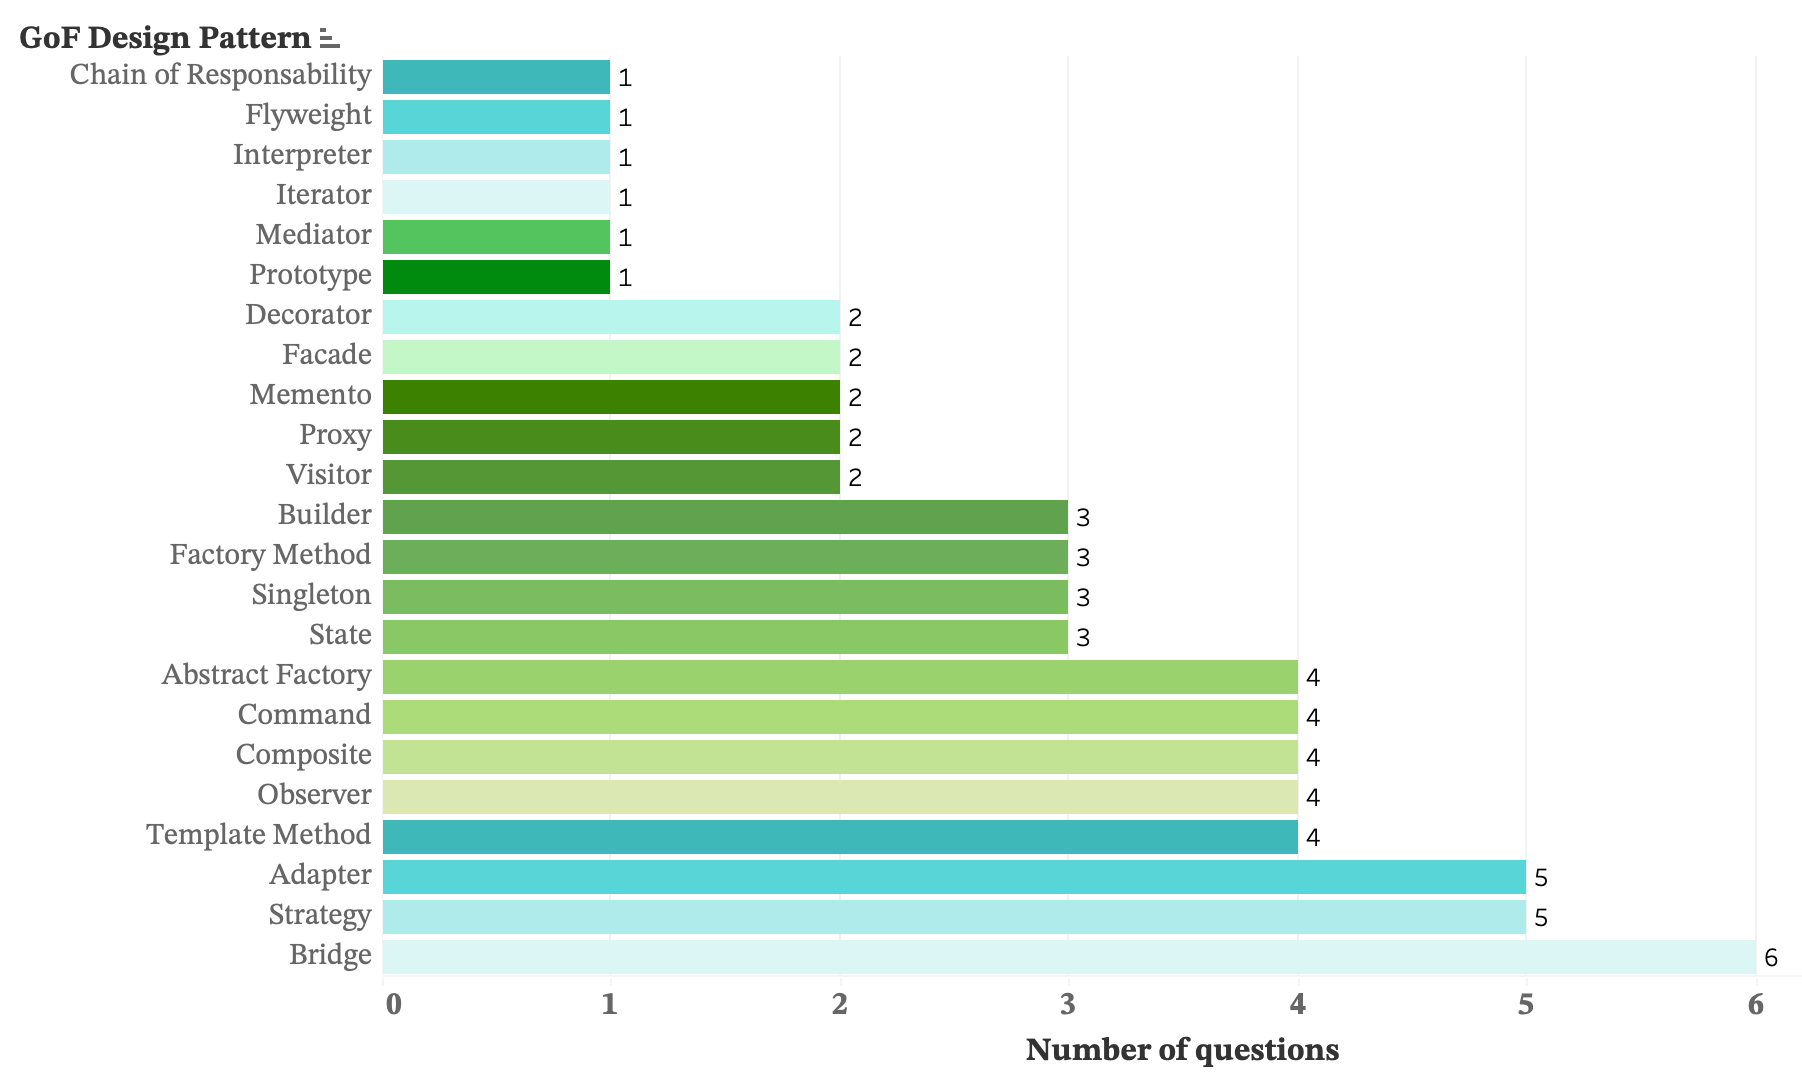
\includegraphics[width=1.0\textwidth]{figures/number-questions.png}
 \objectsource{\objectsourceauthor}
\end{figure}

Considering the pattern categories Figure~\ref{type-patterns}, there are 25 questions about \textit{behavioral} pattern, 22 about \textit{structural} patterns, and 17 about \textit{creational} patterns. 

The question database is reasonably balanced among the pattern categories Figure~\ref{type-patterns}, with many questions covering each. Two questions accepted more than one pattern as a correct answer; we consider anyone right in such cases. Four questions asked for a combination of patterns as an answer; in this case, we considered that the right answer should include all of them.

\begin{figure}[!ht]
\centering
\caption{\centering Categorization of Questions by Design Pattern Types.}\label{type-patterns}
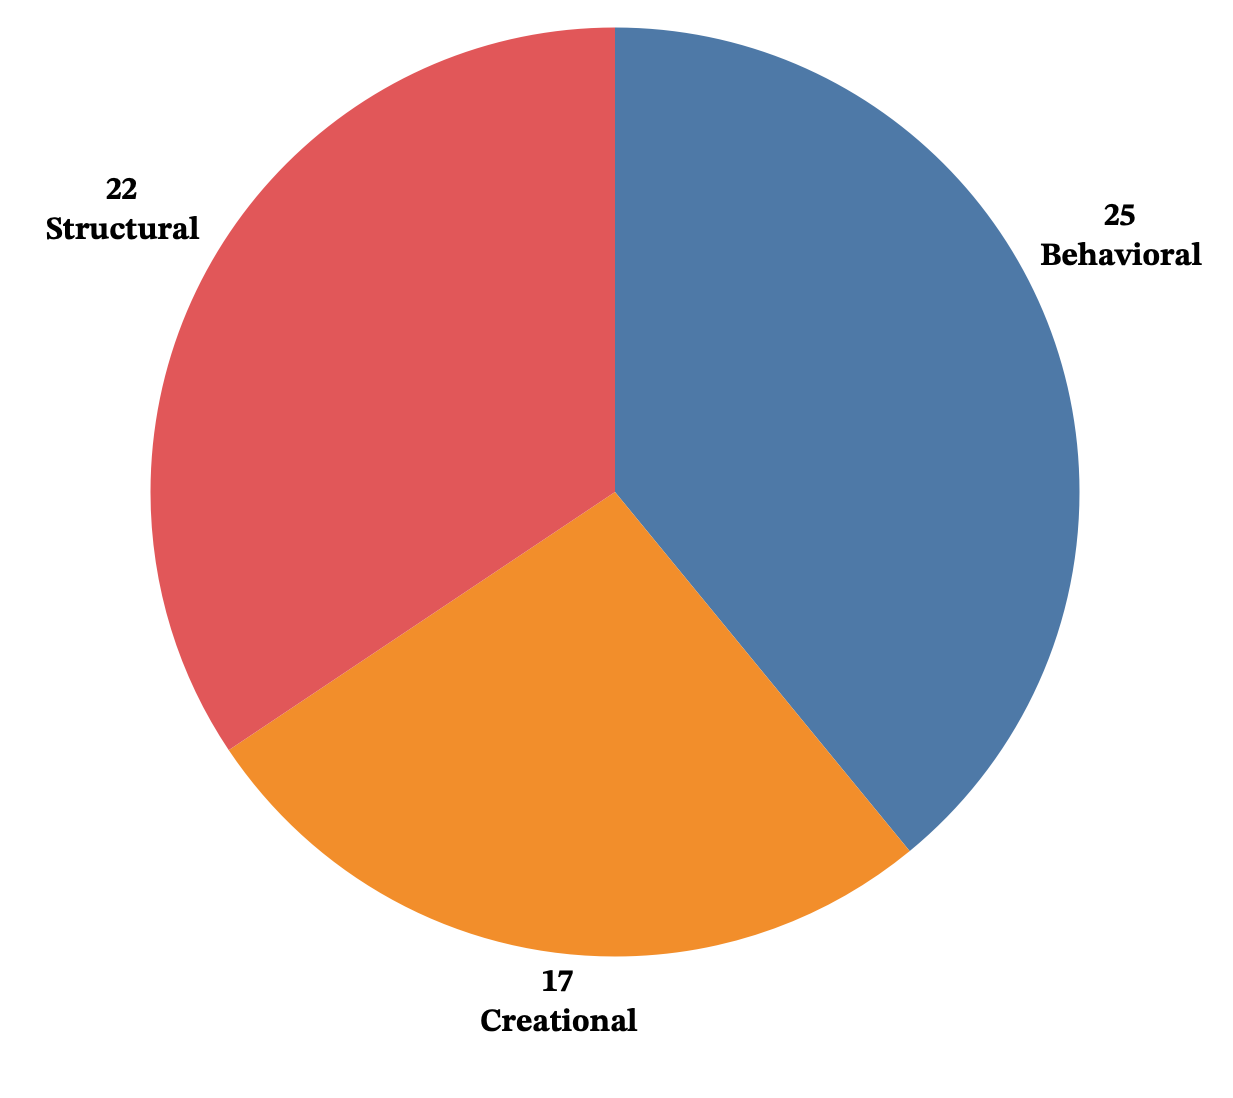
\includegraphics[width=0.70\textwidth]{figures/types-patterns.png}
 \objectsource{\objectsourceauthor}
\end{figure}

\subsection{Prompt Pattern Questions}
In this subsection, we show a question from each criterion from \textbf{\textit{CPS\textsubscript{1}}} to \textbf{\textit{CPS\textsubscript{5}}}  that was input into ChatGPT and their answers.

\MyPara{CPS\textsubscript{1}:}{The answer mentions the context described instead of just giving a generic answer}. In the Prompt \ref{chatgpt-quest:3}, we have a question where the context is about airport control, and in the Output \ref{chatgpt-answers:3}, we have an answer mentioning the context of traffic control. In the link \href{https://chat.openai.com/share/c0b5744b-2357-4396-b107-5995bcee4dc3}{ CPS\textsubscript{1}} we have the prompt executed.

\begin{chatquest}{usercolor}{\chatgptquest[chatgpt-quest:3]}

Pilots of aircraft approaching or departing from the airport control area do not communicate directly with each other. Instead, they speak to an air traffic controller sitting in a tall tower near the airstrip. Without the air traffic controller, pilots would need to be aware of all planes near the airport and discuss landing priorities with a committee of dozens of other pilots. That would likely skyrocket the plane crash statistics.

The turret does not need to control the entire flight. It only exists to enforce constraints on the terminal area because the number of actors involved can be overwhelming for a pilot.

What design pattern can be implemented for this situation?
\end{chatquest}
\begin{chatout}{botbubble}{\chatgptout[chatgpt-answers:3]}
The design pattern that can be implemented for this situation is the Mediator pattern. The Mediator pattern is a behavioral pattern that defines an object and encapsulates how objects interact. It promotes loose coupling by keeping objects from explicitly referring to each other and allowing their interaction to vary independently.
In air traffic control, the controller acts as a mediator between the pilots and ensures that all planes near the airport know each other's positions, speeds, and flight plans. The air traffic controller also decides the landing priorities and enforces constraints on the terminal area to avoid potential collisions.
Using the Mediator pattern, the pilots don't need to communicate directly with each other, and the air traffic controller can handle the overwhelming number of actors involved in the process. This promotes loose coupling and flexibility, allowing the system to vary independently, depending on the number of planes in the area or the complexity of the flight plan.
\end{chatout}

\MyPara{CPS\textsubscript{2}:}{Answer explains the pattern. In Prompt~\ref{chatgpt-quest:4}, no one was asked to explain the pattern; however, in Output~\ref{chatgpt-answers:4}, the patterns \texttt{Decorator}, \texttt{Adapter}, and \texttt{Bridge} are explained. Below is the link as evidence \href{https://chat.openai.com/share/78948591-5150-4621-bd78-16b65bb1922f}{CPS\textsubscript{2}}.}

\begin{chatquest}{usercolor}{\chatgptquest[chatgpt-quest:4]}
Your system has 3 document types, i.e., Letter, Resume, and Laundry List, and 2 document formats, i.e., Microsoft Word and Google Docs. What design patterns could be used to add more document types and formats without adding more code?
\end{chatquest}

\begin{chatout}{botbubble}{\chatgptout[chatgpt-answers:4]}
To add more document types and formats without adding more code, we can use the following design patterns:

\MyParaBold{Decorator Pattern:} We can use the Decorator Pattern to add new functionality to existing document types and formats. For example, suppose we want to add spell-checking functionality to all document types and formats. In that case, we can create a SpellChecker decorator class that wraps around the existing document objects and adds spell-checking functionality without modifying the existing code.

\MyParaBold{Adapter Pattern:} We can use the Adapter Pattern to convert the interface of an existing class to another interface that clients expect. For example, suppose we want to support a new document format that has a different interface from the existing one. In that case, we can create an adapter class that translates the new format's interface to the existing interface.

\MyParaBold{Bridge Pattern:} We can use the Bridge Pattern to separate the abstraction from its implementation, allowing us to change either without affecting the other. For example, suppose we want to support a new document type with a different internal representation from the existing one. In that case, we can create a bridge class that encapsulates the new representation and provides a common interface to the rest of the system.

Using these design patterns, we can add more document types and formats to the system without adding more code to the existing classes. This makes it easier to maintain the system over time, as we can add new functionality and support for new formats without modifying the existing codebase.
\end{chatout}

\MyPara{CPS\textsubscript{3}: }{Answer describes/classes and interfaces to be created to implement the pattern. The coffee ordering system context has multiple types of coffee and condiments that can be combined to create many drink options, shown in Prompt~\ref{chatgpt-quest:5}. However, the challenge is to add all these options to the system to take orders for all available drinks. In the Output~\ref{chatgpt-answers:5}, explain how the classes and interfaces should be created. In the link \href{https://chat.openai.com/share/82b1ca09-7e35-488a-ad93-b95cf8c204b9}{CPS\textsubscript{3}} we have the prompt executed. }

\begin{chatquest}{usercolor}{\chatgptquest[chatgpt-quest:5]}

A coffee ordering system offers various types of coffee, such as House Blend and espresso. Along with coffee, there are also condiments such as Mocha, Milk, Soy, and Milkshakes.
It can be espresso with powdered milk and mocha or house-blended with soy and whipped cream. This system can make quite a few drinks, equivalent to combining all the types and aromas of coffee available.
The problem is adding all these types of drinks to the coffee ordering system so that it takes orders for all available drinks. How to do this?
\end{chatquest}

\begin{chatout}{botbubble}{\chatgptout[chatgpt-answers:5]}

The design pattern that best fits to solve this problem is the Decorator pattern. The Decorator pattern allows for the dynamic addition of behavior to an object at runtime without affecting the behavior of other objects in the same class. In this case, we can dynamically use the Decorator pattern to add condiments to the coffee orders.

We can start by creating an interface or abstract class for the base coffee, representing the common behavior of all types of coffee. Then, we can create concrete classes for each type of coffee, such as House Blend and Espresso. Each of these classes would implement the base coffee interface or abstract class. Next, we can create an abstract decorator class that implements the base coffee interface or abstract class. This decorator class would have a reference to an object of the same type as the base coffee interface or abstract class, and it would dynamically add behavior to this object.

Finally, we can create concrete decorator classes for each type of condiment, such as Mocha, Milk, Soy, and Milkshake. Each of these classes would also implement the decorator abstract class and add the behavior of the corresponding condiment to the object. Using the Decorator pattern, we can create many coffee types and condiment combinations without creating a separate class for each combination. This allows for more flexibility and easier maintenance of the coffee ordering system.
\end{chatout}



\MyPara{CPS\textsubscript{4}: }{Answer describes the methods that should be created to implement the pattern. Based on the Prompt~\ref{chatgpt-quest:1}, Output~\ref{chatgpt-answers:1} describes the classes and methods, showing the structure of the classes and the execution in the link:~\href{https://chat.openai.com/share/77833002-868a-46c1-af63-5b7b5d2c8f1b}{CPS\textsubscript{4}}.}

\begin{chatquest}{usercolor}{\chatgptquest[chatgpt-quest:1]}
You need to develop a crawler to mine the prices of products on grocery store websites. The basic flow of the crawler is to get the URL of the product listing, access each product URL, collect the HTML of the page, parse the HTML to extract the product name, parse the HTML to extract the price and save the info to the database. Each grocery store (e.g., Walmart and Target) has a different HTML structure. 
Write a code snippet (Java or Python) illustrating how you would use the Template Method design pattern to implement this crawler for Walmart and Target.
You don't need to implement the actual miner or parser, I am interested in how you would structure your classes.
\end{chatquest}

\begin{chatout}{botbubble}{\chatgptout[chatgpt-answers:1]}

Sure, I'd be happy to help you with that. Here's an example code snippet in Java that uses the Template Method design pattern to implement the crawler for Walmart and Target:
\begin{lstlisting}[language=Java]
public abstract class GroceryStoreCrawler {
    
    public void crawl(String productListingUrl) {
        String[] productUrls = getProductUrls(productListingUrl);
        for (String productUrl : productUrls) {
            String html = getHtml(productUrl);
            String productName = getProductName(html);
            double price = getPrice(html);
            saveToDatabase(productName, price);
        }
    }
    
    protected abstract String[] getProductUrls(String productListingUrl);
    
    protected abstract String getHtml(String productUrl);
    
    protected abstract String getProductName(String html);
    
    protected abstract double getPrice(String html);
    
    private void saveToDatabase(String productName, double price) {}
}
public class WalmartCrawler extends GroceryStoreCrawler {
    
    @Override protected String[] getProductUrls(String productListingUrl) {}
    
    @Override protected String getHtml(String productUrl) {}
    
    @Override protected String getProductName(String html) {}
    
    @Override protected double getPrice(String html) {}
}
public class TargetCrawler extends GroceryStoreCrawler {
    
    @Override protected String[] getProductUrls(String productListingUrl) {}
    
    @Override protected String getHtml(String productUrl) {}    
    
    @Override protected String getProductName(String html) {}
    
    @Override protected double getPrice(String html) {}
}
\end{lstlisting}
In this code snippet, we have an abstract class, GroceryStoreCrawler, that defines the basic flow of the crawler using the Template Method design pattern. The crawl method is the template method that calls the abstract methods getProductUrls, getHtml, getProductName, and getPrice. These methods are implemented in the subclasses WalmartCrawler and TargetCrawler.Each subclass implements the abstract methods with store-specific code to extract the product URLs, HTML, product name, and price from the store's website. The saveToDatabase method is private and cannot be overridden by the subclasses.
\end{chatout}

\MyPara{CPS\textsubscript{5}:}{answers included a UML diagram to represent the solution. In the Prompt~\ref{chatgpt-quest:2}, the question asks to create a UML diagram that can be illustrated in Output~\ref{chatgpt-answers:2}, which expresses the creation of the Abstract Factory pattern. The execution in the link: \href{https://chat.openai.com/share/02b2ee84-3786-4bf6-bce4-7ec331235c2b}{CPS\textsubscript{5}}.}
\begin{chatquest}{usercolor}{\chatgptquest[chatgpt-quest:2]}

You are developing an online game with 3 kingdoms: Elfs, Humans, and Orcs. The class MapBuilder is responsible for building a map for a kingdom. It randomly positions the castle, the hero, and the army on the map. To make this class generic for any Kingdon, MapBuilder receives an abstract factory as a parameter responsible for creating the kingdom's castle, hero, and army (e.g., Elfs). 
Draw a UML diagram illustrating how the Abstract Factory is used in this example

\end{chatquest}

\begin{chatout}{botbubble}{\chatgptout[chatgpt-answers:2]}
An example UML diagram that illustrates how the Abstract Factory could be used:
\begin{center} 
\begin{tikzpicture}[every node/.style={font=\scriptsize}] 
  \umlclass{MapBuilder}{
    - factory: AbstractFactory
  }{
    + buildMap() : Map
  }

  \umlclass[y=-3.5]{AbstractFactory}{}{
    + createCastle() : Castle \\
    + createHero() : Hero \\
    + createArmy() : Army
  }

  \umlclass[y=-8,type=abstract]{ConcreteFactory}{}{
    + createCastle() : Castle \\
    + createHero() : Hero \\
    + createArmy() : Army
  }

  \umlclass[x=-3, y=-11.5]{ElfCastle}{}{}
  \umlclass[x=0, y=-11.5]{ElfHero}{}{}
  \umlclass[x=3, y=-11.5]{ElfArmy}{}{}

  \umlinherit{AbstractFactory}{MapBuilder}
  \umlinherit{ConcreteFactory}{AbstractFactory}
  \umlinherit{ElfCastle}{ConcreteFactory}
  \umlinherit{ElfHero}{ConcreteFactory}
  \umlinherit{ElfArmy}{ConcreteFactory}
\end{tikzpicture}
\end{center} 
In this diagram, the \textbf{MapBuilder} class depends on the \textbf{AbstractFactory} interface. This means it can work with any concrete factory that implements this interface, allowing it to build maps for any kingdom. 

The \textbf{AbstractFactory} interface defines the methods for creating the castle, hero, and army of a kingdom. Each concrete factory \textbf{ConcreteFactory} implements this interface and provides its own implementation of these methods, creating the specific types of castle, hero, and army for that kingdom.

Finally, each concrete factory creates concrete instances of the castle, hero, and army classes specific to its kingdom. By using the Abstract Factory pattern in this way, we can ensure that the \textbf{MapBuilder} class is decoupled from the specific types of castle, hero, and army that it needs to create, allowing us to easily add new kingdoms in the future without having to modify this class.
\end{chatout}

% ---------------------------------------------------------------------------
% Inicio da Seção Results
% ---------------------------------------------------------------------------
\section{Results}\label{ResulttsPreliminaryStudy}

The questions were sent to ChatGPT (version 3.5) between 2023-03-03 and 2023-04-16. Based on the results, ChatGPT was generally effective in answering our questions, with an overall accuracy rate of 93\%. Most of the questions were in Portuguese, with 31 of the 34 answered correctly, while 21 of the 22 in English were answered correctly. 

The answers have an average of 1033 characters and a standard deviation of 657, varying from a minimum of 247 to a maximum of 3127. Considering the number of words, the average is 155, with a standard deviation of 89, varying from a minimum of 37 to a maximum of 390 words. 

We used the Pearson correlation coefficient to evaluate if the number of words on the question would be related to the number of words in the answer; more details in Figure~\ref{avg-words-patterns}. The value of 0,09 obtained showed that there was no significant relation. 

\begin{figure}[!ht]
\centering
\caption{\centering Average Word Count Analysis of Design Patterns.}
\label{avg-words-patterns}
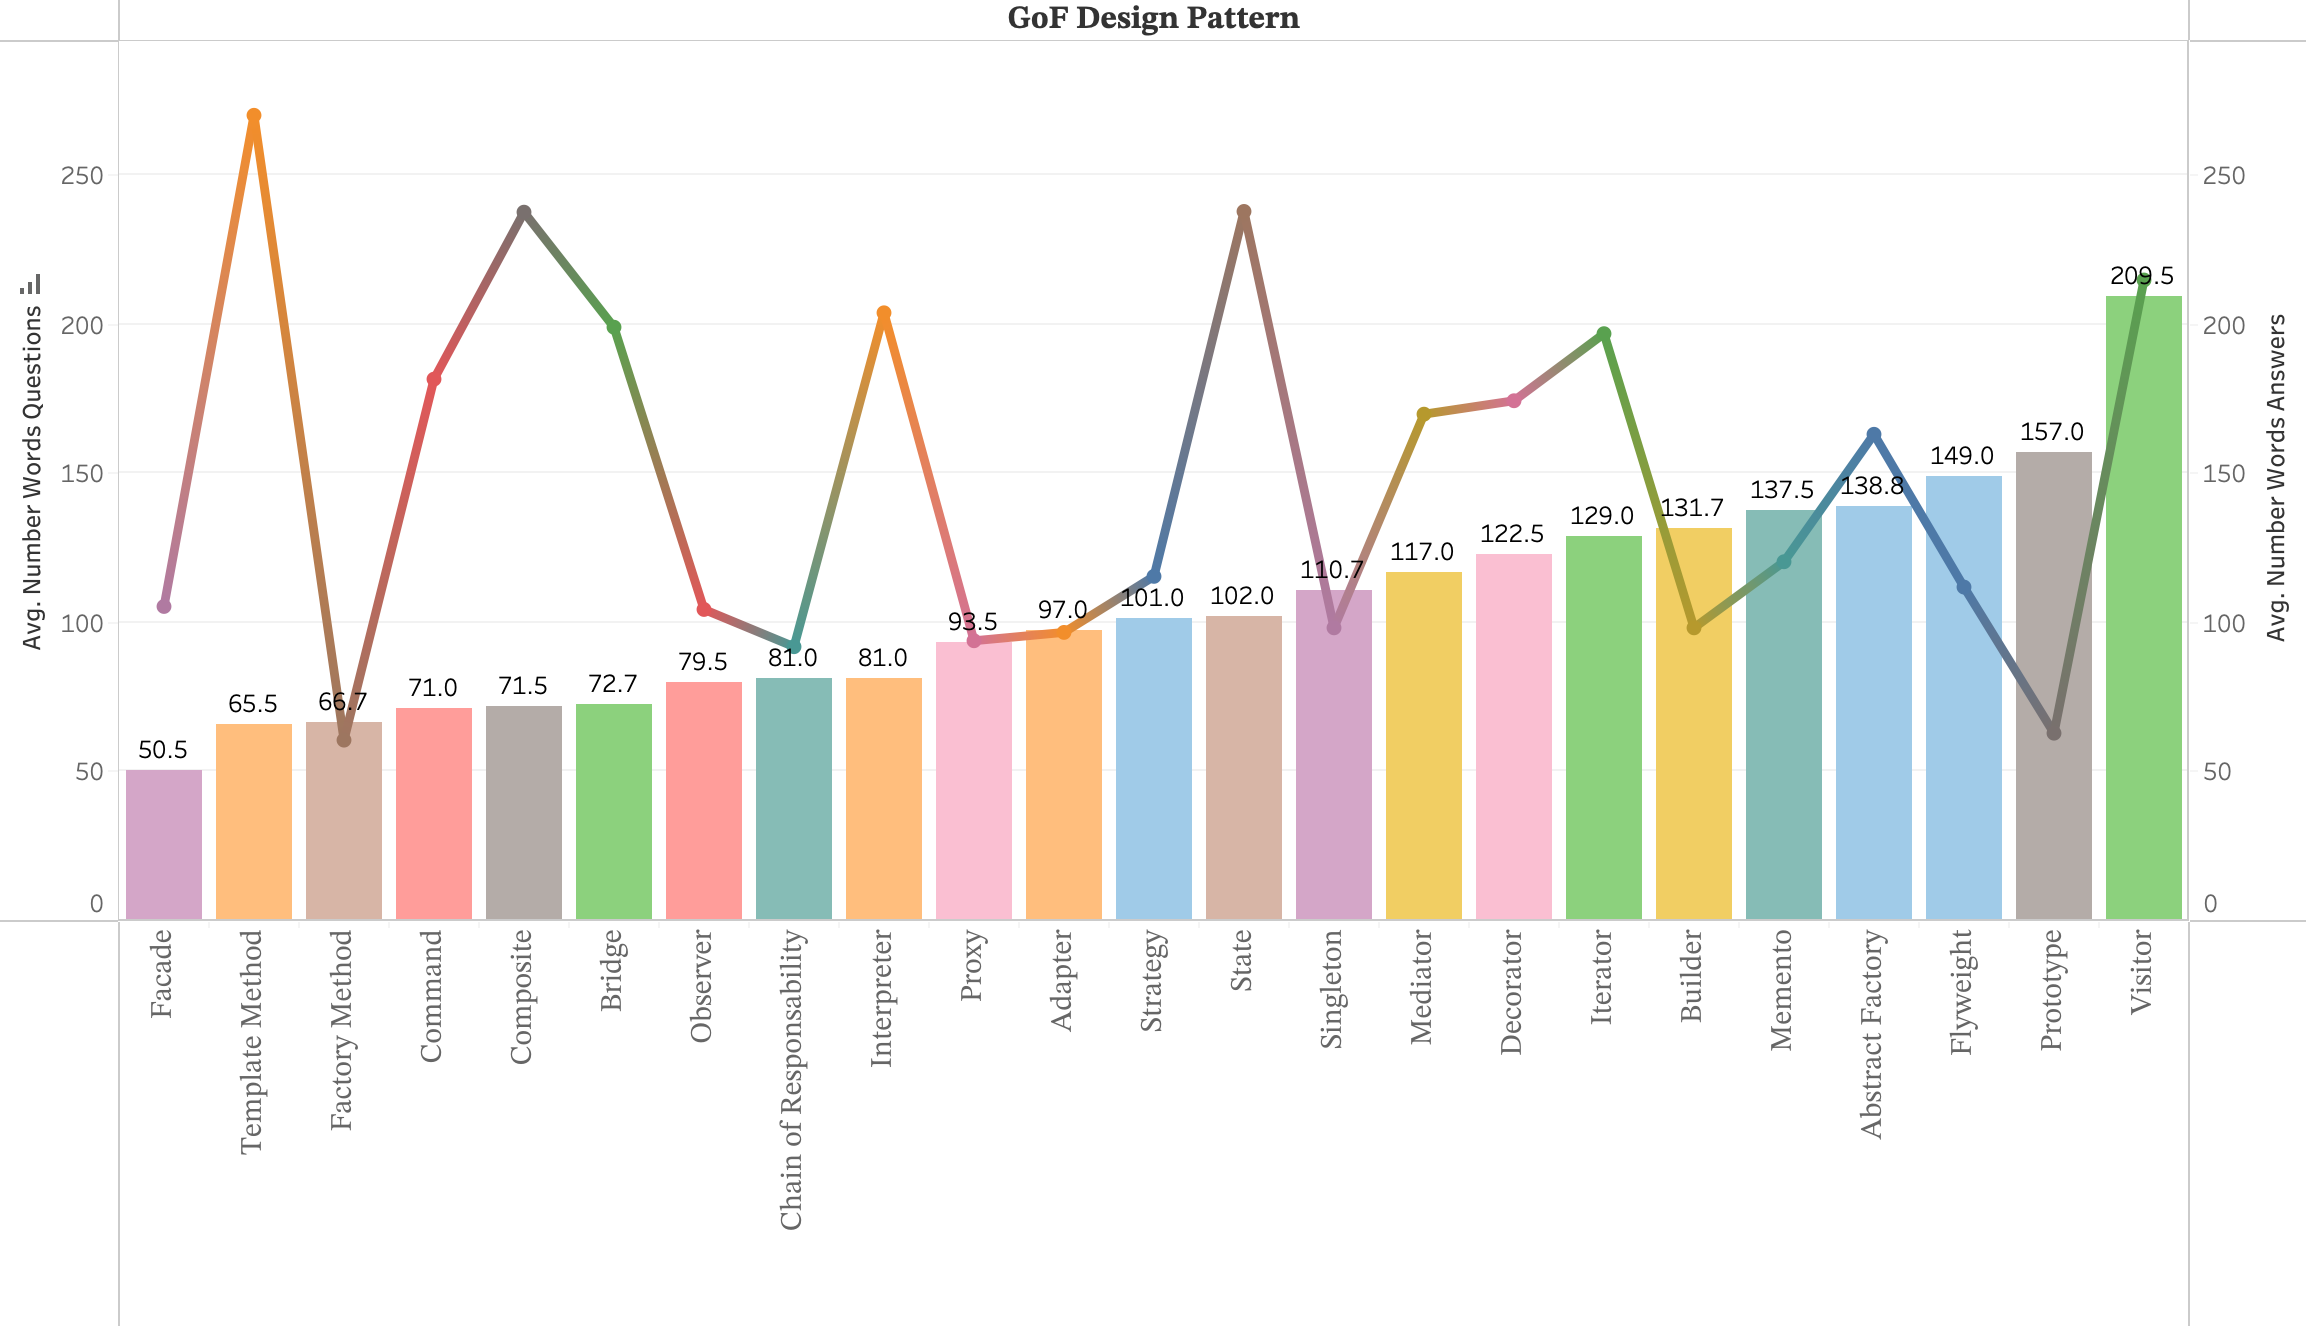
\includegraphics[width=1.0\textwidth]{figures/questions-patterns-avg-words.png}
 \objectsource{\objectsourceauthor}
\end{figure}

\textbf{Information Present in the Answers.} A qualitative analysis evaluated the six criteria proposed in Subsection~\ref{ResearchPreliminaryStudy}. In Table~\ref{table:cps} are the results:

\begin{table}[!ht] 
    \small
    \centering
    \caption{(CPS: Criteria Number),(Rate: Percentage of correct answers for each criterion), (A/Q: Number of correct answers versus total questions), and Criteria Description.}
    \label{table:cps}
    \begin{tabular}{p{0.4in}p{0.5in}p{0.5in}p{4.0in}}       
        \toprule
         \hline
        \rowcolor{gray!19} \textbf{CPS}  & \textbf{Rate} & \textbf{A/Q} & \textbf{Criteria Description}  ~\\ \hline      
        \textbf{\textit{CPS\textsubscript{1}}} & 100\% & 52/52 & Mention the described context instead of just giving a generic answer. ~\\ \hline
        \rowcolor{gray!19} \textbf{\textit{CPS\textsubscript{2}}} & 57.69\% & 30/52 & Explained the Design pattern of the question elaborated.  ~\\ \hline
       \textbf{\textit{CPS\textsubscript{3}}} & 32.69\% & 17/52  & Describe the classes and interfaces that need to be created to implement the pattern. ~\\ \hline
       \rowcolor{gray!19} \textbf{\textit{CPS\textsubscript{4}}} & 26.92\% & 14/52  & Describe the methods that should be created to implement the pattern. ~\\ \hline
       \textbf{\textit{CPS\textsubscript{5}}} & 3.85\% & 2/52  & Include a UML diagram to represent
        the solution. ~\\ \hline
       \rowcolor{gray!19} \textbf{\textit{CPS\textsubscript{6}}} & 0\% & 0/52  & Describe any trade-off or negative consequence in using the proposed pattern. ~\\ \hline
       \bottomrule
    \end{tabular}
    \objectsource{\objectsourceauthor}
\end{table}


\textbf{Assessment of \ac{WA}.} This section presents an analysis of the questions that received a wrong answer (the ID will be used to refer to that question later):

\MyPara{WA\textsubscript{1}} - The question presented Prompt \ref{chatgpt-wa:1}  a problem in creating a solution for reports needing two dimensions: the report type and the report format. While the correct answer was using the Visitor pattern, the tool suggested Strategy.
\begin{chatquest}{usercolor}{\chatgptquest[chatgpt-wa:1]}
A system that generates reports of different types in multiple formats must be developed. The formats include TXT, HTML, PDF, and XML. Report types contain common elements such as titles, subtitles, paragraphs, tables, and information trees. Each report comprises a set of these elements generated from system data. Each type of element that must be present in the report is generated differently according to the format chosen. What design patterns can be used to decouple the code for generating report content from the format in which it will be generated?
\end{chatquest}

In the answer, shown in the Output \ref{chatgpt-wa-answers:1}, one of the dimensions of the question was ignored, and the proposed solution focused only on the report format. This question was originally in Portuguese and can be found in its entirety at the following link  \href{https://chat.openai.com/share/9fca7359-3a95-4032-83a9-f03b45cea436}{WA\textsubscript{1}}.
\begin{chatout}{botbubble}{\chatgptout[chatgpt-wa-answers:1]}

The strategy pattern is the most suitable design for decoupling the code to generate report content from the format in which it will be generated. This standard allows you to define a family of algorithms, encapsulate them, and make them interchangeable, allowing the client to choose the algorithm they want to use at run time. 

In the case of the reporting system, you can create an abstract Report class with methods common to all types of reports, such as generating titles, subtitles, paragraphs, tables, and information trees. Then, concrete classes can be created that extend the Report class for each desired report type, such as TextReport, HTMLReport, PDFReport, and XMLReport.

Finally, a Strategy interface can be created that defines the generateReport() method implemented by the concrete classes of each report format. The Report class can then receive an instance of the report generation strategy in its constructor and call the generateReport() method to generate the report in the desired format. This way, it is possible to decouple the generation of report content from the format in which it will be generated, facilitating the maintenance and extension of the system.
\end{chatout}
   
\MyPara{WA\textsubscript{2}} - The question, shown in the Prompt \ref{chatgpt-wa:2}, asked how the representation of more complex devices could be dynamically created by reusing the behavior of more simple devices that are part of it. While the correct answer was Composite, the given answer was Factory Method, as evidenced in the Output \ref{chatgpt-wa-answers:2}. In this case, the solution described does not help in solving the design problem presented. Follow the Prompt link for more information:\href{https://chat.openai.com/share/15c618ec-4644-4c11-8698-48bfd0a6d177}{WA\textsubscript{2}}.
\begin{chatquest}{usercolor}{\chatgptquest[chatgpt-wa:2]}
Imagine you are developing a system to simulate an industrial IoT environment. The system already provides a few types of virtual devices, and it should be easy to extend with new types of virtual devices, such as cameras, infrared cameras, movement sensors, air-conditioning, and others. Some of these virtual devices are more complex than others. Some exhibit partially the same behaviors as other devices, so it would be a waste of time to code all of them from scratch. Which design pattern is the best to enable dynamically (at runtime) defining new types of devices with varying levels of complexity?
\end{chatquest}
\begin{chatout}{botbubble}{\chatgptout[chatgpt-wa-answers:2]}
The factory method pattern is the design pattern most suitable for dynamically defining new types of devices of varying levels of complexity in an industrial IoT environment.

The Factory Method pattern is a creational pattern that provides an interface for creating objects but allows subclasses to alter the type of objects that will be created. This pattern allows for the dynamic creation of objects at runtime, which makes it an excellent choice for this scenario. Using the Factory Method pattern, you can define a virtual device factory that generates instances of virtual devices based on a specified input. Each virtual device would be a subclass of the virtual device factory, allowing for creating new virtual devices with minimal coding. The virtual device factory can have different methods for creating different types of virtual devices, such as cameras, movement sensors, or air-conditioning units. Each method would take care of the specific configuration and behavior of the corresponding virtual device, while the virtual device factory would handle the general creation process.

By using the Factory Method pattern, you can easily extend the system with new types of virtual devices without having to rewrite the entire codebase. This makes it easier to maintain and update the system over time and add new features and capabilities.
\end{chatout}    
\MyPara{WA\textsubscript{3}} - The question presented in the Prompt \ref{chatgpt-wa:3}, the context of exchanging messages between different cell phone operating systems platforms, handling distinct message formats transparently. While the correct answer was Adapter, the answer was Bridge, as evidenced in the Output \ref{chatgpt-wa-answers:3}. In this case, even if the patterns share some structural similarities, the described solution does not help solve the problem. Follow the Prompt link for more information: \href{https://chat.openai.com/share/97f7ae9f-9403-41e9-9627-8973af95edb8}{WA\textsubscript{3}}.
\begin{chatquest}{usercolor}{\chatgptquest[chatgpt-wa:3]}
An IT Analyst wants to create an application capable of exchanging messages between different mobile platforms, such as an Android sending messages to an iOS, a Windows Phone exchanging messages with an Android, etc. The problem is that each platform implements different ways of receiving messages. She knows that creating multiple methods for each platform would not be a suitable solution because other methods would have to be created if the application needs to include a new platform. Modeling many-to-many relationships can make the system design overly complex. The Analyst then looked for a design pattern to use in the solution. 

Among the GoF standards, you found one that allows you to define an object that encapsulates how a set of objects interact. This pattern promotes loose coupling by preventing objects from referring to each other explicitly and allows you to vary the use of the interaction independently. It acts as an interlocutor between many-to-many relationships, avoiding an explicit reference to objects appropriate to the problem. Is this the behavioral pattern?
\end{chatquest}
\begin{chatout}{botbubble}{\chatgptout[chatgpt-wa-answers:3]}
No, the design pattern described is not a behavioral pattern, but rather a structural pattern called the "Bridge Pattern". The Bridge pattern allows you to decouple an abstraction from its implementation, allowing both to vary independently. In the case described, the Bridge pattern could be used to encapsulate the interaction between different messaging platforms, allowing each one to have its own implementation without affecting the others. This would allow you to add new messaging platforms without affecting the application structure.
\end{chatout}    

\MyPara{WA\textsubscript{4}} - The question presented in the Prompt \ref{chatgpt-wa:4} is an abstract class that is responsible for transparently creating objects corresponding to different types of databases. Concrete subclasses are responsible for instantiating specific connections and queries for each type of database. The correct answer was Abstract Factory, and the given answer was Factory Method, as evidenced in the Output \ref{chatgpt-wa-answers:4}. Even if both are creational patterns, the given answer does not help to solve the problem because it was necessary to create a family of objects for each type of database. Follow the Prompt link for more information: \href{https://chat.openai.com/share/1e475da1-7a8c-4a21-9361-f4549b329230}{WA4}.

\begin{chatquest}{usercolor}{\chatgptquest[chatgpt-wa:4]}
An application must be able to manipulate different types of databases transparently to classes requiring data access services. Initially it will be necessary to provide support for XML and SQL databases, however new types may be added in the future. The proposed solution is as follows:

1. An abstract class (DB) will be responsible for instantiating an object corresponding to the desired database type. This will be done through the static getDB() method, which will return an object from one of its concrete subclasses according to the parameter (type) passed.

2. The object created in the previous step will instantiate connections and queries corresponding to the type of DB created; if an XML DB has been instantiated, only XML queries and XML connections will be instantiated. If a SQL DB has been instantiated, only SQL queries and SQL connections will be instantiated.

Which design pattern was used in the proposed solution?
\end{chatquest}
\begin{chatout}{botbubble}{\chatgptout[chatgpt-wa-answers:4]}
The design pattern used in the proposed solution is the Factory Method design pattern. The Factory Method is a creation pattern that defines an interface for creating objects in a superclass but allows subclasses to change the type of objects that will be created. It is used when a class cannot anticipate the class of objects it must create.

In the proposed solution, the DB abstract class acts as the Creator class of the Factory Method pattern. The static getDB() method is the factory method that creates database objects (product objects) corresponding to the desired database type. These objects are returned as instances of one of the concrete DB subclasses, depending on the parameter (type) passed.

Furthermore, the proposed solution also predicts that each database object created (concrete DB) will instantiate connections and queries corresponding to the type of database created. This conforms to the Factory Method pattern as it allows subclasses to change the type of objects that will be created.

Thus, the proposed solution follows the Factory Method standard, allowing different types of objects (databases) to be created transparently for classes that require data access services.
\end{chatout}    

% ---------------------------------------------------------------------------
% Inicio da Seção Discussion
% ---------------------------------------------------------------------------
\section{Discussion}\label{DiscussionPreliminaryStudy}

This section discusses the obtained results, answering each research question. We also point out some limitations of the present study.

\begin{itemize}
    \item  \textbf{\textit{RQPS\textsubscript{1}}} - How is the success rate of the AI-assisted tool in suggesting design patterns?\label{sec5sub1}
    
    The study showed an efficient result with 93\% correct answers in 56 questions. We highlight that the questions the AI-assisted tool provided the correct answer in the four questions that required a combination of patterns as any answer to the question by choosing the right pattern; the relevant factors that point to the usage of that specific pattern need to be identified in the context description. We also highlight that in the four questions that required a combination of patterns as an answer, the AI-assisted tool provided the correct answer.

    ChatGPT performance can be considered good compared to other works that proposed more specific techniques for pattern suggestion~\cite{Hussain2019automated, Naghdipour2023Semi}. Consequently, it can be considered a suitable assisting tool for developers, which can describe the design scenario in their application and receive suggestions from the tool.

     \item  \textbf{\textit{RQPS\textsubscript{2}}}  - Do elements provided in the answer of the AI-assisted tool help in the pattern implementation?\label{sec5sub2}

     One positive point is that all responses mentioned the problem's context instead of just pointing to the pattern and providing a generic explanation. Around one-third of the answers also provided the names of the classes and interfaces that should be created in that case. Additionally, around one-quarter described the methods that should be created. Few answers, only 2, also provided UML diagrams with the structure that should be used.

    Most of the answers, but not all, brought a more theoretical explanation of the pattern, which can be useful in case the developer is unfamiliar with the pattern. A piece of important information not present in any of the answers is the trade-off in using the suggested pattern since knowing possible bad consequences is important to making design decisions.
    
    To avoid bias, the questions used in this study were not modified; however, we acknowledge that if we explicitly included what information we wanted in the answer, the tool would include it. We did some exploratory experiments on some of the questions, rephrasing them to ask explicitly for some missing information. As a result, the missing information was included correctly in the new answers. That fact highlights the importance of how the questions are formulated, a new disciple called prompt engineering~\cite{White2023}.  

    \item  \textbf{\textit{RQPS\textsubscript{3}}} - In questions where the wrong pattern is pointed, does the AI-assisted tool answer mislead the developers?\label{sec5sub3}

    We analyzed the four questions that received wrong answers to see if there was any inconsistency or ambiguity in their formulation. All authors agreed that they were clearly described, and there was no doubt about the correct answer. For all the patterns that were the correct answer for these questions, there is at least another question with the same pattern answered correctly.

    In the case of \textbf{\textit{WA\textsubscript{1}}}, the answer given by ChatGPT considered the described context partially, and the Strategy implementation that it described could be evolved to a Visitor. However, in \textbf{\textit{WA\textsubscript{2}}}, \textbf{\textit{WA\textsubscript{3}}}, and \textbf{\textit{WA\textsubscript{4}}}, the answer leads to a way that does not solve the problem. The answers are assertive and well-described, and we believe can readily be accepted by a less experienced developer. Because of that, we advise that the answers given by an AI-assisted tool should be reviewed and understood instead of being blinded implemented. In other words, a professional should be responsible for its analysis and adoption.
    
    We also noticed that some of these questions used terms and expressions closely connected to other patterns. So, we suggest avoiding expressions like ``family of algorithms'' or ``composite objects'' that can drive the tool to a specific pattern.
    
\end{itemize}

\MyParaBold{Limitations of Design Patterns Selection}\label{sec5sub4}

Our study focused only on ``Gang of Four'' (GoF) design patterns, which are well-known and widely used in the software development community. The performance of ChatGPT may differ for other design patterns that are newer and have less material available.

Our study was conducted in a controlled setting using preexisting questions. These questions were formulated by teachers with software design knowledge, focused on scenarios suitable for applying one of the patterns, and included all the necessary information relevant to direct the answer to one of the patterns. Using such a tool in a real project would require skills to identify the relevant forces in the scenario and formulate them properly~\cite{White2023}. Asking which pattern should be used might force the choice of one pattern in cases where none is suitable.

\subsection{Section Summary}

Section 3 of this research presents a preliminary study focused on selecting design patterns using generative AI tools. This chapter begins by describing the study's objectives, which aim to evaluate the effectiveness of generative AI, particularly GPT models, in accurately identifying and recommending suitable design patterns for specific software development problems.

The study's methodology is outlined, detailing how existing questions related to design pattern selection were posed to ChatGPT. The responses were then analyzed to assess their accuracy and relevance. The chapter includes a comprehensive analysis of the results, showcasing the potential and limitations of AI tools.

Key findings from the study highlight that while the generative AI tool was able to provide accurate and relevant design pattern recommendations in most cases, there were instances where the responses were less precise, indicating areas for further improvement in the AI's training and prompt engineering.

Overall, Section 3 sets the stage for further exploration by demonstrating the initial feasibility of using generative AI tools in design pattern selection and providing valuable insights into their current capabilities and potential areas for enhancement.